

\documentclass[12pt]{article}

\usepackage{sbc-template}

\usepackage{graphicx,url}

\usepackage[utf8]{inputenc}
\usepackage[brazil]{babel}
\usepackage{float}
\usepackage{graphicx}
\usepackage[most]{tcolorbox}
\usepackage{graphicx,url}
\usepackage[export]{adjustbox}

\sloppy

\title{Concepção de uma Arquitetura Móvel para Identificação de Anomalias Cardíacas}

%\author{Rodrigo Leal\inst{1}, Cidrônio Oliveira\inst{1}, Ismael Pereira\inst{2}, Francisco Airton Silva\inst{1}}

%\address{Universidade Federal do Piauí
 %(UFPI)\\
 %Picos -- PI -- Brasil
% \nextinstitute
 %Universidade Federal do Piauí (UFPI)\\
 % Teresina -- PI -- Brasil
%}
\begin{document} 

\maketitle

\begin{abstract}
  Abnormal changes in heart impulses can mean serious illnesses that need frequent monitoring. Traditional metering solutions present recognized precision, however they become expensive when patients decide to be frequently examined. This paper presents an analysis of some low-cost mobile technologies for heart rate monitoring, such as the Mi Band 2 bracelet and Instant Heart Rate applications, 4Free Blood Pressure and ICare Health Monitor. The metrics analyzed were: practicality, measurement environment, data manipulation, platform, precision and cost. In terms of precision, the Mi Band 2 bracelet was close to 92 \%. Based on this result, this paper proposes a distributed system capable of identifying cardiac anomalies with the Mi Band 2 bracelet.
\end{abstract}
 
\begin{resumo}
  Mudanças anormais nos impulsos cardíacos podem significar enfermidades graves que requerem monitoramento frequente. As soluções tradicionais de medição apresentam uma conceituada precisão, porém custosas quando realizadas com frequência. Esse artigo mostra uma análise de algumas tecnologias móveis de baixo custo para monitoramento de impulsos cardíacos, como o bracelete Mi Band 2 e aplicativos Instant Heart Rate, 4Free Blood Pressure e ICare Monitor de Saúde. As métricas analisadas foram: praticidade, ambiente de medição, manipulação dos dados, plataforma, precisão e custo. Em termos de precisão, o bracelete Mi Band 2 chegou próximo de 92\%. Baseado nesse resultado, o artigo apresenta uma proposta de um sistema distribuído capaz de identificar anomalias cardíacas com o bracelete Mi Band 2.
\end{resumo}

\section{Introdução}

O coração é um órgão vital para funcionamento do corpo humano. Diversas enfermidades podem afetar o fluxo cardíaco saúdavel \cite{AE}. Existem várias técnicas para o monitoramento dos impulsos cardíacos, a citar as tradicionais como Holter, Eletrocardiograma e Oxímetro; além de inovações como a pulseira Mi Band 2 e aplicativos móveis, tais como \textit{Instant Heart Rate}, \textit{4Free Blood Pressure} e \textit{ICare} Monitor de Saúde.

As ferramentas tradicionais possuem reconhecida precisão, porém, tem custo oneroso para cardiopatas e registro não contínuo. Contudo, inovações podem proporcionar mobilidade e baixo custo. Este artigo propõe a concepção de uma sistema distribuído capaz de monitorar e identificar anomalias cardíacas de forma móvel, automática e contínua.

\section{Ferramentas de Monitoramento Cardíaco} \label{sec:firstpage}

O monitoramento cardíaco pode ser feito com diversos métodos. Nas tecnologias tradicionais, destacam-se: o Eletrocardiograma (ECG), Holter e Oxímetro. O ECG é referência para diagnóstico não invasivo de arritmias\footnote{Diretriz da interpretação do ECG em repouso – Sociedade Brasileira de Cardiologia.}, apesar de ter atividade limitada fora do ambiente hospitalar \cite{massot}. O método de Holter faz o registro do ECG por períodos diários do paciente \cite{holter}. A Tabela 1 e 2 mostram um estudo de custo do ECG e Holter, respectivamente, em feveireiro desse ano, na cidade de Teresina (PI).

\begin{table}[h!]
    \begin{minipage}{.5\linewidth}
      \caption{Preço do ECG.}
      \centering
      \begin{adjustbox}{max width=\textwidth}
        \begin{tabular}{*{14}{|c}|}%%{|c|c|}
            \hline
              \textbf{Clínica} & \textbf{Preço}\\
              \hline
              Clínica 1 & R\$ 60.00 \\
              \hline
              Clínica 2 & R\$ 58.00 \\
              \hline
              Clínica 3 & R\$ 54.35 \\
             \hline
        \end{tabular}
        \end{adjustbox}
    \end{minipage} 
    \begin{minipage}{.5\linewidth}
      \caption{Preço de Holter.}
      \centering
        \begin{adjustbox}{max width=\textwidth}
          \begin{tabular}{*{14}{|c}|}%%{|c|c|}
          \hline
          \textbf{Clínica} & \textbf{Preço}\\
          \hline
          Clínica 1 & R\$ 200.00 \\
          \hline
          Clínica 2 & R\$ 230.00 \\
          \hline
          Clínica 3 & R\$ 174.00 \\
          \hline
        \end{tabular}
        \end{adjustbox}
    \end{minipage} 
\end{table}

O Oxímetro é um método apto a medir a frequência cardíaca de forma instantânea a um preço variável de R\$ 250,00\footnote{http://www.medjet.com.br/busca/oxímetro} \cite{garbey} . Ele deve ser acoplado a regiões do corpo com pouca resistência à luz e em ambientes com apropriada luminosidade\footnote{https://sbpt.org.br/espaco-saude-respiratoria-oximetria-de-pulso/}.

As tecnologias móveis agrupam a pulseira Mi Band 2\footnote{ http://www.mi.com/en/miband2/} e aplicativos móveis. A Mi Band 2 é uma nova geração de dispositivos vestíveis carregados com funções de medição de dados cardíacos e calóricos. Os aplicativos \textit{Instant Heart Rate}, \textit{4Free Blood Pressure} e \textit{ICare} Monitor de Saúde funcionam monitorando mudanças suaves na coloração da pele. A iluminação e adequação retilínia entre dedo e câmera devem se fazer presentes para a realização das medições com esses aplicativos\footnote{http://www.techtudo.com.br/dicas-e-tutoriais/noticia/2011/05/aprenda-monitorar-seus-batimentos-cardiacos-usando-o-seu-celular.html}.

\section{Trabalhos Relacionados}

Nesta seção são mostradas pesquisas que proporam melhorias nos métodos de monitoramento tradicionais. Xu et al (2016) apresentaram uma tecnologia baseada em análise de bioimpedância, com maior praticidade em comparação ao ECG. Li et al (2017) apontam a criação de um modelo para leitura do ECG em longos períodos, com uso de \textit{software}. 

Massot et al (2015) mostram a criação de um sensor de atividade cardíaca capaz de enviar sinais via \textit{Wi-Fi}. Todos os trabalhos divulgaram praticidade em relação às técnicas anteriores, registro contínuo e mobilidade (respectivamente), porém sem discussão de outras métricas como apresentado no presente estudo.

\section{Comparação entre Tecnologias Móveis}\label{sec:figs}

Esta seção apresenta um comparativo entre as tecnologias recentes. As métricas analisadas foram: praticidade (facilidade na obtenção dos dados), ambiente de medição (local apropriado), manipulação dos dados (manuseio dos dados colhidos), plataforma (sistemas operacionais suportados), precisão (acurácia da técnica) e custo (desembolso necessário).

Para se medir a precisão, foram feitas trinta medições divididas igualmente em três faixas etárias (adolescentes, adultos e idosos). Os valores de referência foram obtidos com auxílio de um estetoscópio\footnote{http://www.enciclomedica.com.br/estetoscopio/}. A Figura 1 apresenta o cálculo da acurácia. Os resultados de cada aplicativo foram confrontados com o valor do estetoscópio. A acurácia média de um aplicativo foi obtida a partir da média aritmética simples das precisões particulares.

\begin{figure}[H]
\centering
% Comando para colocar borda na imagem.
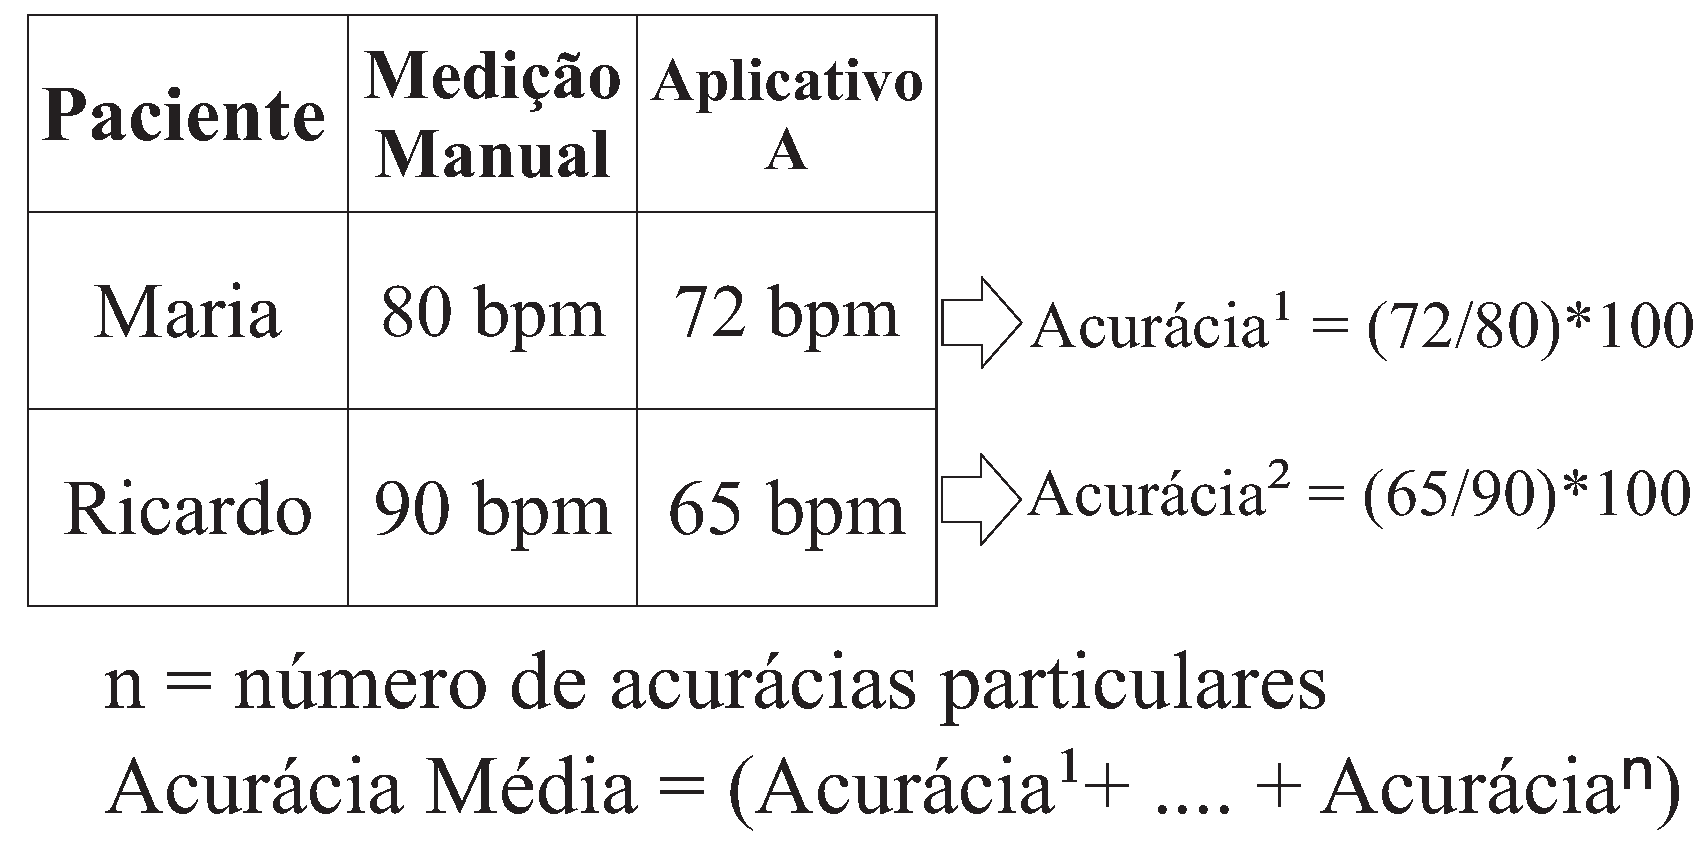
\includegraphics[width=.34\linewidth, frame]{explanation}
\caption{Cálculo da Acurácia Média.}
\label{fig:exampleFig1}
\end{figure}

As figuras abaixo apresentam as acurácias levantadas das tecnologias sobre cada faixa etária. A pulseira Mi Band 2 é representada nos gráficos como MB 2, \textit{Instant Heart Rate} como IHR, \textit{4Free Blood Pressure} como 4Free e \textit{Icare} Monitor de Saúde como ICare.

\begin{figure}[H]

\minipage{0.24\textwidth}
  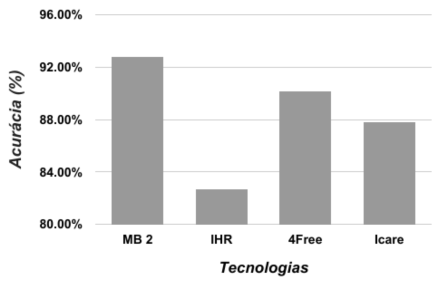
\includegraphics[width=\linewidth]{Grafico1}
  \caption{Adolescentes.}\label{fig:awesome_image1}
\endminipage\hfill
\minipage{0.24\textwidth}
  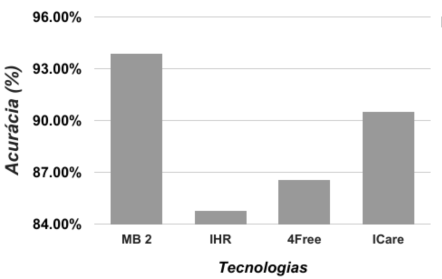
\includegraphics[width=\linewidth]{Grafico2}
  \caption{Adultos.}\label{fig:awesome_image2}
\endminipage\hfill
\minipage{0.24\textwidth}%
  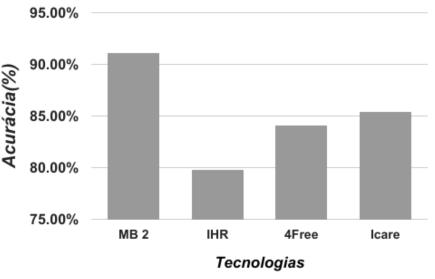
\includegraphics[width=\linewidth]{Grafico3}
  \caption{Idosos.}\label{fig:awesome_image3}
\endminipage

\end{figure}

Foi aplicado o método estatístico ANOVA\footnote{http://www.est.ufpr.br/ce003/material/cap7.pdf} na comparação entre as medições das três amostras. A Figura 5 apresenta o resumo da análise. O gráfico mostra a relação entre os intervalos e médias de acurácia das tecnologias. A margem de acerto da Mi Band 2 é superior às demais, enquanto que o \textit{4Free Blood Pressure} e \textit{ICare} Monitor de Saúde apresentam linhas de representação sobrepostas, indicando medições aproximadas.

\begin{figure}[H]
\centering
% Comando para colocar borda na imagem.
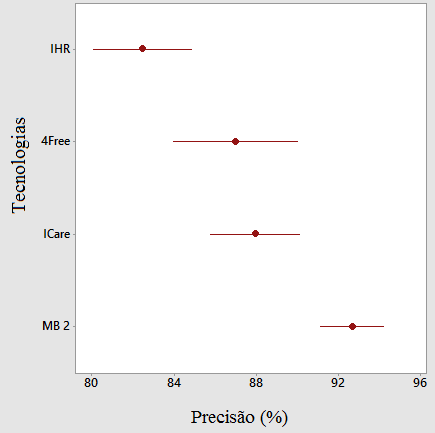
\includegraphics[width=.29\linewidth, frame]{Grafico4.png}
\caption{Comparação entre Intervalos e Médias de Precisão.}
\label{fig:exampleFig5}
\end{figure}

O \textit{Icare} Monitor de Saúde possui uma menor amplitude em relação ao \textit{4Free Blood Pressure}, ou seja, um variância reduzida. A Tabela 3 mostra o paralelo entre as tecnologias nas métricas definidas. Pode-se ver uma diferença variável entre as acurácias. De forma inversamente proporcional às acurácias, o \textit{Instant Heart Rate} mostra mais de 10 milhões no Google Play\footnote{https://play.google.com/store?}, já o \textit{4Free Blood Pressure} tem pouco mais de 100.000, enquanto que o \textit{ICare} Monitor de Saúde detem pouco mais de 1 milhão de \textit{downloads}.

\begin{table}[h!]
  \centering
  \caption{Comparativo entre Tecnologias Móveis de Baixo Custo.}
  \label{tab:label_test}
  \begin{adjustbox}{max width=\textwidth}
  \begin{tabular}{*{7}{|c}|}%%{|c|c|c|c|c|c|c|}
  \hline
  Tecnologia & Praticidade & Ambiente de Medição & Manipulação dos Dados & Acurácia & Plataforma & Custo \\
  \hline
  MB 2 & Alta & Qualquer & Sim & 92\% & Android, iOS e MIUI & R\$ 350.00\footnote{http://www.americanas.com.br/produto/19689776?oferta=31393638393737392e32313239363333323030303133352e4e4557. Acesso em 23.02.2017} \\
  \hline
  IHR & Alta & Alguns & Não & 82\% & Android, iOS & Gratuito \\
  \hline
  4Free & Alta & Alguns & Não & 87\% & Android, iOS & Gratuito \\
  \hline
  ICare & Alta & Alguns & Não & 88\% & Android, iOS & Gratuito \\
  \hline
\end{tabular}
\end{adjustbox}
\end{table}

\section{Arquitetura}

Com base na análise apresentada acima, esta pesquisa tem o objetivo de desenvolver uma ferramenta que recebe o monitoramento realizado pelo bracelete Mi Band 2 e processa os dados à fim de prover um diagnóstico de possíveis anomalias cardíacas.

A Figura 6 mostra a arquitetura proposta composta por três módulos que são: Coletor, Receptor e Infraestrutura de Armazenamento. O Coletor designa a pulseira Mi Band 2 para leitura dos impulsos cardíacos; o Receptor faz o acompanhamento e interpretação das frequências cardíacas por meio de aplicativo \textit{Android}; e a Infraestrutura de Armazenamento trata-se do ambiente on-line para mantimento e acesso  dos dados cardíacos pela equipe médica.

\begin{figure}[H]
\centering
% Comando para colocar borda na imagem.
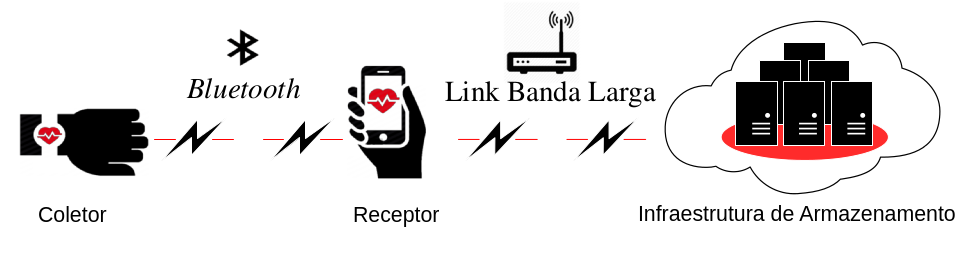
\includegraphics[width=.40\linewidth, frame]{Arquitetura.png}
\caption{Arquitetura Móvel para Identificação de Anomalias Cardíacas.}
\label{fig:exampleFig5}
\end{figure}

\section{Conclusão}


Mudanças anormais nos batiemntos cardíacos podem significar enfermidades graves. O custo de exames de monitoramento tradicionais em clínicas varia conforme o método. O valor médio para um cardiopata que realiza quatro exames anuais fica por volta de R\$ 229,40 (ECG) a R\$805,40 (método Holter). A pulseira Mi Band 2 se torna uma alternativa vantajosa por ter um custo baixo, mobilidade e precisão durante a leitura.

%A pulseira Mi Band 2 tem alta precisão (92\%), praticidade, independência do cenário de medição e um custo reduzido, tornando-se mais apropriado ao uso hospitalar dentre os aplicativos. O aplicativo \textit{ICare} Monitor de Saúde pode ser um recurso alternativo, com uma precisão aproximada de 87\% e baixa variação.

A Arquitetura apresentada busca prover um diagnóstico rápido e com uso de tecnologia de baixo custo, a pulseira Mi Band 2.  Sendo assim possível encontrar variações e anomalias que podem auxiliar médicos e pacientes no tratamento.

\bibliographystyle{sbc}
\bibliography{sbc-template}

\end{document}